%\chapter{Introduction}

\section{Background}

\begin{itemize}
 \item General importance
\end{itemize}

At nanoscale, theories describing energy transfer in macroscale objects break down and new phenomena emerge. Striking examples are, for example, the observation of thermal conductance quantization \cite{schwab00}, divergence of thermal conductivity in two-dimensional carbon \cite{xu14}, 100-fold reduction in nanowire thermal conductivities compared to the bulk values \cite{} and break-down of the Planck blackbody radiation law in the near-field \cite{}. In addition to leading to new understanding of physics, these phenomena offer new ways to engineer the thermal properties of materials.

%Physically, such phenomena arise from the reduced dimensionality, wave interference effects, increased geometric scattering rates, reduced internal scattering and near-field effects appearing in nanoscale structures. 
\begin{itemize}
 \item Phase-change memory
 \item Electronics
 \item Thermoelectrics
 \item Thermal therapy
\end{itemize}

\begin{itemize}
 \item Half the world energy production is wasted as heat ($\sim 10^{13}$ TW), efficient reclaiming would 
 \item Thermal rectifiers could act as energy harvesters
 \item Half the power consumed by data centers is spent on cooling, most limiting factor in performance
 \item Race to increase operating frequency stopped as local energy dissipation hit 100 W/cm$^2$, hotter than a hot plate
\end{itemize}



\section{Scope and objectives}
%The second law of thermodynamics essentially dictates that in absence of external agents influencing the system, energy is always transferred from hot to cold, thereby smoothing any temperature differences. 
This doctoral thesis aims at (i) presenting new insight into energy transfer mechanisms in nanoscale structures, and (ii) developing new computational methods for theoretical description of thermal transfer in atomic scale systems. We limit our scope to heat transfer by lattice vibrations and electromagnetic radiation, thereby excluding both electronic conduction and convection.

%The scope of this work is to investigate and develop new computational methods for (i) thermal conduction by lattice vibrations and electrons in nanoscale structures, and (ii) thermal radiation in inhomogeneous environments such as a mirror cavity. We only consider solid materials and therefore convection, which is a major energy transfer mechanism in fluids and gases containing free atoms or molecules carrying heat, is outside the scope of this work. %Below, we review the mo

\begin{figure}
\begin{center}
 %\includegraphics[width=8.6cm]{pics/schwab00_fig3.ps}
 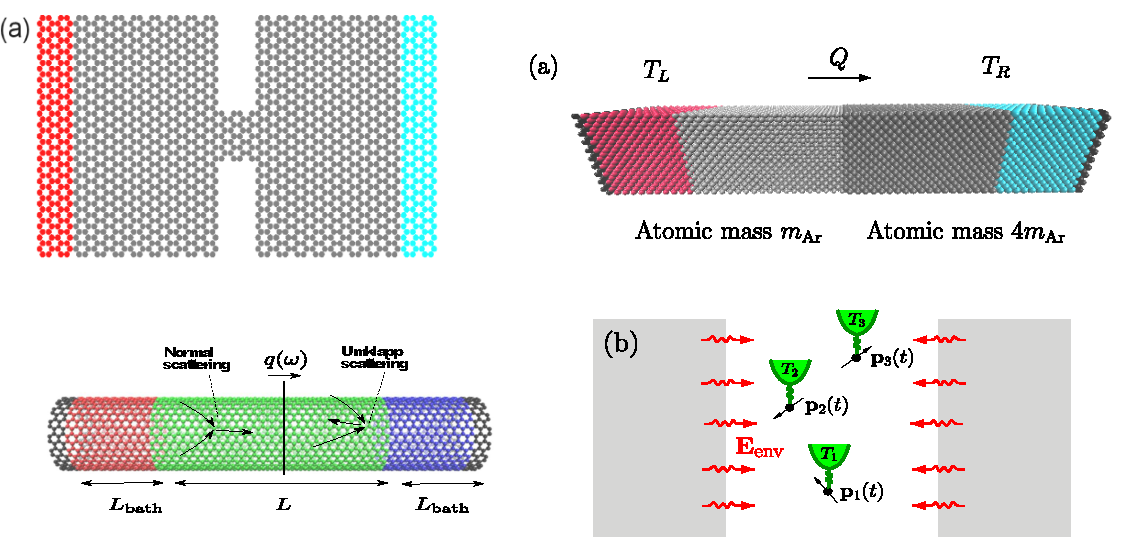
\includegraphics[width=.99\columnwidth]{pics/systems.pdf}
 \caption{Schematic illustration of some of the systems studied in this thesis. (a) Constriction in graphene. (b) Planar interface between two mass-mismatched face-centered cubic lattices. (c) Carbon nanotube. (d) Oscillating dipoles in a cavity.}
\label{fig:intro_systems}
\end{center}
\end{figure}

Some of the systems studied in this work are illustrated in Fig. \ref{fig:intro_systems}. We investigate interference effects and the effect of temperature on energy transfer and non-equilibrium temperature profiles in constrictions in two-dimensional lattices such as graphene, depicted in Fig. \ref{fig:intro_systems}(a). We develop computational methods to determine the spectral distribution of heat current (heat current as a function of vibrational frequency) and apply the method to investigate the role of anharmonic phonon scattering on the thermal conductance of a planar interface depicted in Fig. \ref{fig:intro_systems}(b). We also apply the spectral heat current method to determine the phonon mean free paths in carbon nanotubes [Fig. \ref{fig:intro_systems}(c)] from non-equilibrium simulations. Finally, we present a quantum Langevin equation-based approach on calculating electromagnetic energy transfer rates between oscillating dipoles and apply the theory to investigate the role of an inhomogeneous environment on electromagnetic energy transfer between nanoparticles.



%\begin{itemize}
% \item Interference and anharmonicity effects in constrictions
% \item Energy transfer mechanisms and the role of anharmonicity in interfacial energy transfer
% \item 
%end{itemize}

To set the research topics into more general context, we briefly review below the most prominent energy transfer phenomena appearing in nanoscale systems.

% Energy transfer between and inside bodies generally occurs by three mechanisms: conduction, radiation and convection \cite{}. 
%The energy transfer generally occurs by three mechanisms: conduction, radiation and convection \cite{}. Thermal conduction, which is the dominant mechanism in solids, is energy transfer inside a given body and occurs through (i) the microscopic interactions between the atoms and molecules constituting the body and, in case of metals, (ii) movement of free electrons. In fluids and gases, energy is transferred not only by conduction but also by the net motion of the energy-carrying molecules themselves, a process known as convection. As an example, the familiar law that hot air rises above the cold air is convection. Finally, energy can be transmitted by electromagnetic waves, i.e., thermal radiation. Unlike conduction and convection, thermal radiation does not require any mediating medium to carry energy: this is best exemplified by the thermal radiation from the Sun.

%The scope of this work is to investigate thermal conduction by lattice vibrations and electrons in nanoscale crystalline solids and thermal radiation between nanoparticles. In crystalline solids, lattice vibrations form propagating collective modes, the quanta of which are known as phonons. Below, we briefly review the main phenomena characteristic of thermal conduction in nanoscale. Detailed theory of lattice dynamics is presented in Chap. XXX.

% when the size of the structure or the scale of observations reaches nanoscale.

%\subsection{Experimental observations of }

%\begin{itemize}
% \item Interference, particles versus waves
% \item Boundaries and interfaces
% \item Ballistic versus diffusive, coherence
%\end{itemize}


\section{Vibrational energy transfer in nanoscale systems}

\subsection{Nanoscale phenomena}

%\subsection{Anomalous conductivity}

%Thermal conduction in macroscopic systems is traditionally described using Fourier's law \cite{}. The law states that the heat flux at any given point is proportional to the temperature gradient at the same point. The theory is, therefore, completely local and based on the definition of local temperature, whose changes are dictated by the diffusion equation. Diffusion equation predicts, for example, that the information of a temperature perturbation can propagate infinitely fast in the system, which is in direct contradiction to special relativity. Fourier's theory must, therefore, ultimately break down.

Thermal conduction in macroscopic systems is traditionally described using Fourier's law \cite{}, which states that the heat flux at any given point is proportional to the temperature gradient at the same point. The theory leads, however, to the unphysical phenomenon that a local temperature perturbation can propagate infinitely fast \cite{chen}, in direct contradiction to special relativity. This indicates that Fourier's theory must ultimately break down in nanoscale.

The microscopic theory for thermal conduction was developed by Rudolf Peierls in 1929 \cite{}. Understanding that collective lattice vibrations (phonons) carry heat in crystalline solids, he proposed that thermal resistivity arises from the scattering of phonons from lattice imperfections and other phonons. These scattering mechanisms existing in any non-ideal material at non-zero temperature give rise to a finite phonon mean free path, characterizing the average distance between scattering events. At length scales smaller than the mean free path, phonons can travel without scattering and Fourier's fully local theory must be invalid. At length scales much larger than the mean free path, on the other hand, the heat carriers are expected to propagate diffusively and heat transfer is well described by Fourier's theory.

This expected transition to the ''Fourier limit'' in sufficiently large systems was questioned in 1997 by the simulations of S. Lepri \textit{et al.} \cite{lepri97}, who found that the Fourier limit is never achieved in one-dimensional chains: the thermal conductivity was found to diverge as a function of system length. Later studies have elaborated on the divergence using various methods \cite{narayan02,mai07}. It is, however, still debated \cite{} if any physical system such as a nanowire can be treated as a one-dimensional object and could therefore exhibit the divergence. Some experiments have claimed to have observed the divergence in silicon nanowires \cite{yang10}, but the evidence remains inconclusive. In two-dimensional materials such as graphene, similar divergence is expected, and recent experiments and simulations for graphene have suggested this to be the case \cite{xu14}. %\citepub{cnt}

\begin{figure}
\begin{center}
 %\includegraphics[width=8.6cm]{pics/schwab00_fig3.ps}
 \includegraphics[width=8.6cm]{pics/schwab00_fig3.pdf}
 \caption{Thermal conductance measured as a function of temperature by Schwab \textit{et al.} \cite{schwab00}. In their experimental setup, heat was transferred through four nanowires with four acoustic modes in each carrying the heat. The measured conductance at low temperature is therefore $G=16g_0$, where $g_0$ is the conductance quantum. Reprinted with permission from Ref. \cite{schwab00}.}
\label{fig:intro_schwab}
\end{center}
\end{figure}

In systems smaller than the phonon mean free path, on the other hand, Fourier's law is automatically invalid due to the scattering-free propagation of heat carriers. Such bullet-like transport of phonons is called ballistic transport, contrasting with the diffusive transport of Fourier-like systems. The most striking example of ballistic transport is the thermal conductance quantization, predicted theoretically by Rego and Kirczenow in 1998 \cite{rego98}. Their calculations showed that at sufficiently low temperatures, where phonon scattering is minimal and only the lowest-frequency phonon modes can be excited, thermal conductance through a narrow constriction is an integer multiple of the thermal conductance quantum. The thermal conductance quantum, which is analogous to the quantum of electrical conductance, is independent of any material properties and only depends on temperature and Planck's constant. The predicted quantization was observed experimentally in 2000 by Schwab \textit{et al.} \cite{schwab00} (see Fig. \ref{fig:intro_schwab}), thereby indirectly confirming also the existence of ballistic transport.

In addition to the mean free path, there is another internal length scale governing heat transfer, the phonon wavelength. In devices smaller than or of the same size as dominant phonon wavelength, interference effects appear. Interference effects have enabled designing acoustic reflectors with novel applications in enhancing the optical-mechanical coupling \cite{fainstein13} and phonon lasing \cite{maryam13}. Wavelength-related effects are also useful in thermal engineering: as an example, Kim \textit{et al.} were able to reduce the thermal conductivity of InGaAs alloy (which naturally scatters short-wavelength phonons due to point defects) by introducing nanoparticles acting as scatterers for mid-to-long-wavelength phonons \cite{kim06}. %\citepub{fpu}\citepub{fpu2}\citepub{gf} % Other examples of interference

In a nanoscale system with relatively long internal phonon mean free paths, the material surfaces and interfaces play an important role in thermal conduction. At rough surfaces, for example, phonons are scattered into all directions, which strongly suppresses the heat flow. The resulting reduced thermal conductivity has been noted to be responsible for the moderately high thermoelectric figure of merit of Si nanowires \cite{hochbaum08}. At material interfaces, the mismatch in the acoustic properties of the materials inevitably scatters phonons.  This contact resistance between dissimilar materials can act as a major bottleneck limiting the extraction of heat from electronic devices, thereby hindering their performance \cite{}. Many methods have been suggested to reduce the thermal resistance between materials, including chemical functionalization \cite{hopkins11,kaur14}, external pressure \cite{shen11,chalopin12}, and heat-mediating thin films \cite{}. %\citepub{spectral}\citepub{twinning}

% Relation to the thesis
Concepts such as phonon interference, ballistic transport, mean free paths, and interface scattering appear throughout this thesis. In Publications \cp{fpu}, \cp{fpu2}, and \cp{gf}, we explore the interference effects exhibited in thermal conduction through nanoscale constrictions and reveal intricate interference patterns in local nonequilibrium temperature profiles. We also show how such patterns vanish at higher temperatures due to increased scattering. In Publication \cp{spectral}, we present detailed maps of the contributions of different vibrational frequencies to thermal conduction across a mass-mismatched interface, improving thereby the understanding of heat transfer mechanisms at interfaces and presenting guidelines for future thermal engineering of high-conductance interfaces. Publication \cp{cnt} presents a non-equilibrium method for determining the mean free paths of phonons in carbon nanotubes, supplying a theoretical description of the ballistic-diffusive crossover in one-dimensional systems. In Publication \cp{twinning}, we perform ''thermal engineering'' and demonstrate the existence of minimun thermal conductivity at a certain twinning period length in a silicon nanowire. The minimun arises from the maximal blocking of bulk-like scattering-free propagation of phonons through the nanowire by the periodically repeating twinning boundaries.


\subsection{Theoretical background}

%As discussed in Chap. 1, propagating lattice vibrations carry heat in crystalline solids, and the quanta of such propagating vibrations are called phonons. The theoretical description is based essentially on the equations of motion for the atoms in the solid. Because fully quantum description does not easily allow for accounting for non-linear dynamics, which play an essential role in any system with non-negligible phonon-phonon interactions, the discussion below treats the atomic dynamics classically. 

%\begin{itemize}
% \item The goals of this work
%\end{itemize}
The theoretical description of lattice heat transfer is based on the dynamical equations of motion for the atoms constituting the lattice. The equations of motion are generally dictated by the Hamiltonian \cite{ziman}
\begin{equation}
 \ca{H} = \sum_{i=1}^N \frac{\bb{p}_i^2}{2m_i} + \ca{V}(\bb{r}_1,\dots,\bb{r}_N). \label{eq:th_hamiltonian}
\end{equation}
Here $\br_i$, $\bp_i$, and $m_i$ are the position, momentum and mass of atom $i$, respectively. The total number of atoms (which can also be infinite) is denoted by $N$. The first term of Eq. \eqref{eq:th_hamiltonian} is the total kinetic energy of the atoms and the second term $\ca{V}$ is the interatomic potential energy responsible for the interatomic interactions. The choice of the potential energy function $\ca{V}$ is crucial for an accurate description of the lattice dynamics and, consequently, of energy transfer. Models for $\ca{V}$ used in this work are explained in detail in Sec. \ref{sec:th_interatomicpotential}.

Applying Hamilton's equations of motion $\dot{\br}_i=\partial H/\partial \bp_i$ and $\dot{\bp}_i=-\partial \ca{H}/\partial \br_i$ \cite{fetter} gives Newton's law
\begin{equation}
 m_i \ddot{\br}_i = \bb{F}_i, \label{eq:th_eom}
\end{equation}
where the force acting on atom $i$ is
\begin{equation}
 \bb{F}_i = - \frac{\partial \ca{V}}{\partial \bb{r}_i}. \label{eq:th_force}
\end{equation}
For given initial conditions $\br_i(0)$ and $\dot{\br}_i(0)$, Eq. \eqref{eq:th_eom} determines the time evolution of atomic trajectories. To model energy transfer, the equations of motion are supplemented by terms accounting for coupling to external heat baths. In this work, we mostly employ Langevin heat baths that turn the equations of motion into stochastic equations and ensure that the long-term atomic trajectories correctly sample the non-equilibrium statistical ensemble. Langevin theory is presented in Sec. \ref{sec:th_langevin}.

Equation \eqref{eq:th_eom} generally describes the motions of atoms and molecules in solid, gas, and liquid systems. In solids, the atoms vibrate close to their equilibrium positions $\br_i^0$ and one can gain more insight into the lattice dynamics by only considering small displacements from the equilibrium. The positions $\br_i^0$ are defined by the condition of zero force:
\begin{equation}
 \left. \frac{\partial \ca{V}}{\partial \br_i} \right|_{\br_j=\br_j^0 \quad \forall j} = 0. \label{eq:th_zeroforce}
\end{equation}
Assuming that the atoms remain close to the equilibrium positions, one can expand the potential energy in Taylor series in terms of the displacements $\bu_i=\br_i-\br_i^0$:
\begin{equation}
 \ca{V} = \ca{V}_0 + \frac{1}{2} \sum_{i,j} \sum_{\alpha,\beta} u_i^{\alpha} K_{ij}^{\alpha \beta} u_j^{\beta}  + \ca{O}(u^3). \label{eq:th_V_taylor}
\end{equation}
Here the Cartesian coordinate directions $\alpha,\beta \in \{x,y,z\}$ have been written explicitly for clarity and the second-order term is proportional to the ''force constant''
\begin{equation}
 K_{ij}^{\alpha\beta} = \left. \frac{\partial^2 \ca{V}}{\partial u_i^{\alpha} \partial u_j^{\beta}} \right|_{\bu=\mathbf{0}}. \label{eq:th_K_def}
\end{equation}
The first-order derivative term in \eqref{eq:th_V_taylor} vanished based on Eq. \eqref{eq:th_zeroforce} and the last term is of third order in displacements.

In the case that the third-order term can be neglected, employing Eq. \eqref{eq:th_V_taylor} in the equation of motion \eqref{eq:th_eom} gives the system of linear equations
\begin{equation}
 m_i \ddot{u}_i^{\alpha} = - \sum_j \sum_{\beta} K_{ij}^{\alpha\beta} u_j^{\beta}.
\end{equation}
Following standard eigenmode theory \cite{fetter}, the eigenmodes of the system can be found by diagonalizing the matrix $D_{ij}^{\alpha\beta} = (m_i\omega^2 \delta_{ij}\delta
^{\alpha\beta}-K_{ij}^{\alpha\beta})$. In a periodically repeating crystal, the eigenmodes can be labeled by the wavevectors $\bb{q}$ belonging to the first Brillouin zone \cite{ziman} and the branch $p \in \{1,\dots,3N_{\textrm{cell}}\}$, where $N_{\textrm{cell}}$ is the number of atoms in the unit cell. The eigenmodes are called phonon modes, while phonons are the discrete quanta of eigenmode occupation. The eigenfrequencies $\omega(\bb{q},p)$ form the phonon bandstructure, specifying the relation between the wavevectors and frequencies supporting propagating phonon modes. As an example, Fig. \ref{fig:th_nika} shows the phonon bandstructure of graphene, a single monolayer of graphite.

\begin{figure}
\begin{center}
 \includegraphics[width=8.6cm]{pics/nika09_fig3.pdf}
 \caption{Phonon bandstructure of graphene, calculated using the valence force field method \cite{nika09}. The two-dimensional bandstructure is plotted along one-dimensional lines between special points in graphene reciprocal lattice, denoted by $\Gamma$, $M$ and $K$. Because graphene has two atoms per unit cell, there are altogether six phonon branches. The three branches that have vanishing frequencies at the $\Gamma$ point are called longitudinal acoustic (LA), transverse acoustic (TA) and out-of-plane acoustic (ZA). The optical modes LO, TO and ZO are labeled similarly. Reprinted with permission from Ref. \cite{nika09}.}
\label{fig:th_nika}
\end{center}
\end{figure} 

When the anharmonic part in Eq. \eqref{eq:th_V_taylor} is neglected, the phonon eigenmodes are exact eigenmodes of the system and cannot dissipate their energy, giving rise to infinite thermal conductivity \cite{ziman}. The anharmonic terms give rise to phonon-phonon scattering \cite{ziman}, which is the primary phonon decay mechanism in crystalline solids at high temperatures. In Publications \cp{fpu}, \cp{fpu2}, \cp{spectral}, \cp{cnt}, and \cp{twinning}, we have employed classical molecular dynamics simulations fully accounting for anharmonic scattering. In \citepub{gf}, anharmonic effects are mimicked by the self-consistent heat bath model \cite{bolsterli70}, allowing for the inclusion of quantum statistics as well. These methods are explained in more detail below in Chap. XXX.



%As noted by Kapitza already in 1930s \cite{}, carrier scattering at interfaces between materials also gives rise to thermal resistance. Even in the absence of defects, 

% Point contacts \cite{bartsch12}

% Contact resistance is a bottleneck
% Material properties increasingly dominated by interfaces

% Interfaces

% Superlattices, phonon mirrors

% While there is convincing evidence from numerical simulations that the Fourier limit is always achieved in three-dimensional systems \cite{saito10,wang10}, this seems not to be the case in one- or two-dimensional systems. Numerical simulations \cite{lepri97,mai07} and hydrodynamical theory \cite{} suggest that the thermal conductivity in one-dimensional systems diverges in a power-law fashion as a function of system length, but clear experimental demonstration of the divergence has not been achieved so far. In two-dimensional systems, thermal conductivity is expected to diverge logarithmically \cite{}. Recent experiments claim to have observed the divergence in graphene \cite{xu14}.

%\subsection{Thermal boundary resistance}

%\subsection{Thermal engineering}

\section{Electromagnetic energy transfer in nanoscale}

\subsection{Near-field energy transfer}
Accelerating charges are known to emit electromagnetic radiation \cite{}. Because the electrons and nuclei in any solid material undergo thermal (and quantum) fluctuations, all materials therefore emit electromagnetic radiation carrying heat. In 1900, Max Planck \cite{planck00a} studied the radiation emitted by a blackbody and gave birth not only to quantum theory but also to Planck's blackbody radiation law, which has since been observed to describe, for example, the spectrum of cosmic microwave background radiation at the accuracy of XXX.

Planck's law inherently suggests that the total power of the emitted radiation is independent of the distance from the object. This follows from the assumption that only propagating waves contribute to the energy density. Close to the material surface, solution of Maxwell's equations gives, however, also rise to evanescent electromagnetic fields localized at a distance of a few wavelengths from the object \cite{polder71}. One can then envisage placing another object sufficiently close to the radiating body so that the evanescent fields can induce motion of charges in the added object, leading to energy transfer by the evanescent fields. Planck's law therefore breaks down at very small distances. 

The breakdown in Planck's law was first observed by Hargreaves \cite{hargreaves69}, who found an enhancement in the heat transfer rate between two chromium layers as the layers were separated by subwavelength gap. The theoretical calculation for the exact enhancement rate was carried out by Polder and van Hove \cite{polder71}, and consequently near-field enhancement effects were predicted in numerous geometries \cite{loomis94,pendry99,carminati99,shchegrov00,mulet01,volokitin01}. In the last decade, advances in experimental techniques have allowed for very precise measurements of near-field enhancement rates \cite{}, confirming the experimental predictions. Near-field effects are now routinely used in thermal microscopy \cite{majumdar99,muller-hirsch99,kittel05,kittel08}. They are also expected to give rise to engineering applications in, e.g., infrared thermophotovoltaics \cite{dimatteo01,narayanaswamy03,laroche06} and building narrow-band infrared antennas \cite{greffet02}. 

\begin{figure}
\begin{center}
 %\includegraphics[width=8.6cm]{pics/schwab00_fig3.ps}
 \includegraphics[width=8.6cm]{pics/shchegrov00_fig1.pdf}
 \caption{The spectral energy density of electromagnetic field (arbitrary units) close to a SiC surface at distances of (a) $1$ mm, (b) $2$ $\mu$m, and (c) $100$ nm. At the distance of 100 nm, the spectral energy density is dominated by the surface phonon polariton at frequency $\omega=178.7$ Trad/s, resulting in essentially monochromatic energy emission. Inset show the spectral energy densities plotted in semilogarithmic scale. Reprinted with permission from Ref. \cite{shchegrov00}.}
\label{fig:intro_shchegrov}
\end{center}
\end{figure} 

Near-field effects are particularly strong for materials supporting evanescent surface waves decaying at both sides of the surface \cite{shchegrov00}. The surface waves arise from the coupling between the electromagnetic field and either the free electrons (surface plasmon polaritons) or transverse optical phonons (surface phonon polaritons). While surface plasmon polaritons can only be thermally excited in metals at temperatures much higher than room temperature, surface phonon polaritons can contribute to thermal transfer in polar semiconductors even at room temperature. To demonstrate the large contribution of surface waves, Fig. \ref{fig:intro_shchegrov} shows the theoretically calculated \cite{shchegrov00} spectral energy density of the electromagnetic field at various distances from a SiC surface.

Similarly, near-field effects strongly increase the spectral density of the electromagnetic field in the vicinity of nanoparticles made of a polar material. Consequently, heat transfer between two nanoparticles in vacuum is found to strongly increase at small distances \cite{domingues05}. In practice, however, the required nanoparticle distances for efficient heat transfer may be too small, so for practical applications it would be necessary to engineer the thermal conductance to be higher. From the theory of dipole emission, it is well known that the optical-mechanical coupling can be enhanced by orders of magnitude in an inhomogeneous environment such as in a mirror cavity \cite{novotny}. This raises the question, if the interparticle heat transfer rate between particles could be enhanced by cavity. This question was investigated and answered in positive in \citepub{dipole}.

\subsection{Theoretical background}

\subsubsection{Field due to an oscillating dipole}

The theoretical description of electromagnetic energy transfer between oscillating dipoles is based on Maxwell equations \cite{novotny}. In the non-magnetic materials with no free charges that are considered in this work, the electromagnetic fields arise from the fluctuating electric polarization fields inside the bodies, and the Maxwell equations for the electric field $\bE(\br,t)$ and magnetic field $\bb{H}(\br,t)$ read \cite{novotny}
\begin{subequations}
\begin{align}
  \nabla \times \bE(\br,t) &= - \mu_0 \frac{\partial \bb{H}(\br,t)}{\partial t}, \label{eq:th_maxwell1} \\
  \nabla \times \bb{H}(\br,t) &= \varepsilon_0 \frac{\partial \bb{E}(\br,t)}{\partial t} + \frac{\partial \bb{P}(\br,t)}{\partial t}, \label{eq:th_maxwell2} \\
   \nabla \cdot \bb{H}(\br,t) &= 0, \\
   \nabla \cdot \bb{E}(\br,t) &= 0.
\end{align}
\end{subequations}
Equation \eqref{eq:th_maxwell2} shows that a temporal change in the polarization density $\bb{P}(\br,t)$ gives rise to a magnetic field, which in turn induces an electric field according to Eq. \eqref{eq:th_maxwell1}. The induced electromagnetic field carries energy flux, whose magnitude and direction are given by the Poynting vector $\bb{S}(\br,t)=\bb{E}(\br,t)\times \bb{H}(\br,t)$ \cite{novotny}.

To determine the amount of energy radiated by a fluctuating dipole, one needs to solve for the electric and magnetic fields emitted by the dipole current density distribution $\bb{j}(\br',t)=\partial \bb{P}(\br,t)/\partial t$. As shown in detail in Ref. \cite{novotny}, the electric field is given in frequency-domain by 
\begin{equation}
 \tilde \bE(\br,\omega) = \tilde \bE_0(\br,\omega) + i \omega \mu_0 \int_V d\mathbf{r}' \mathbb{G}(\br,\br';\omega) \tilde{\bb{j}}(\br',\omega). \label{eq:th_Etilde}
\end{equation}
Here $\tilde{\bE}_0(\br,\omega)$ is the electric field arising from sources other than the oscillating dipoles, volume $V$ encloses the dipoles and $\mathbb{G}(\br,\br';\omega)$ is the electromagnetic Green's dyadic, which is essentially a $3\times 3$ matrix. The Green's dyadic can generally be decomposed into the free-space and scattered parts as
\begin{equation}
 \mathbb{G}(\br,\br';\omega ) = \mathbb{G}_0(\br,\br';\omega ) + \mathbb{G}_s(\br,\br';\omega ). \label{eq:th_G_decomp}
\end{equation}
The first term, which corresponds to the field radiated by the dipole in absence of any scattering events, is \cite{novotny}
\begin{equation}
 \mathbb{G}_0(\br,\br';\omega) = \left[\mathbf{I}_{3\times 3} + \frac{1}{k_0^2} \nabla \nabla \right] \frac{e^{ik_0|\br-\br'|}}{4\pi|\br-\br'|}.
\end{equation}
Here $k_0=\omega/c$ is the wavevector in vacuum and $\mathbf{I}_{3\times 3}$ is the $3\times 3$ identity matrix. The second term $\mathbb{G}_s(\br,\br';\omega)$ accounts for the scattering of the emitted field by the inhomogeneities in the environment such as reflecting walls. The decomposition \eqref{eq:th_G_decomp} is useful, because the two terms behave differently for $\br\to \br'$: the dyadic $\mathbb{G}_0$ diverges for $\br\to \br'$, but the scattering part $\mathbb{G}_s$ is smooth \cite{novotny}. Having the expression \eqref{eq:th_Etilde} for the electric field, the magnetic field $\tilde{\bb{H}}(\br,\omega)$ can be solved from the first Maxwell equation \eqref{eq:th_maxwell1}, and one can calculate the Poynting vector $\bb{S}$.

\subsubsection{Fluctuational electrodynamics}

To calculate the energy transfer between bodies, we need an equation specifying the relation between the fluctuations in dipole moments and the material's optical properties and temperature. The traditional approach is the fluctuational electrodynamics (FED) theory pioneered by Rytov \cite{rytov} and Lifshitz \cite{lifshitz55}. The core of FED is the fluctuation-dissipation relation \cite{novotny,agarwal75_1}
\begin{equation}
 \langle \tilde{\bp}(\omega)\tilde{\bp}(\omega')^T\rangle = 4\pi \hbar \delta(\omega+\omega')  \textrm{Im}[\alpha(\omega)] \left[f_B(\omega,T)+\frac{1}{2} \right], \label{eq:th_fed_fdt}
\end{equation}
which is used to relate the stochastic fluctuations in the local dipole moment $\tilde{\bp}(\omega)$ (which is the local dipole density integrated over a small volume) to the imaginary part of the dipole polarizability dyadic $\alpha(\omega)$ and dipole temperature $T$. 

While Eq. \eqref{eq:th_fed_fdt} has been used to successfully calculate energy transfer rates in various situations \cite{}, there are two arguments supporting a more microscopic approach. First, because FED relies on an effective medium property, the local polarizability, applying the theory to very small systems requires great care. It was noted only recently by Manjavacas and Abajo de Carc\'ia \cite{manjavacas12} that the fluctuation-dissipation relation connecting the polarization to the polarizability must be modified when local radiative corrections become important to ensure that non-absorbing particles do not emit thermal radiation. Starting from a more microscopic theory would make it possible to avoid resorting to effective medium parameters in the formulation. Second, one can envision  when the optical phonons responsible for electromagnetic radiation cannot be considered to be decoupled from the acoustic phonons responsible for ''phonon radiation''. In such cases, it is necessary to describe the full lattice dynamics and its coupling to the electromagnetic field microscopically. 

In Publication \cp{dipole}, we developed such a microscopic generalization of fluctuational electrodynamics, basing the description of thermal fluctuations on writing quantum Langevin equations for the microscopic dipole oscillations. By starting from the microscopic equations of motion, we could straightforwardly derive expressions for heat transfer rates between dipoles in an inhomogeneous environment in full analogy to the phononic case treated in \citepub{gf}, directly accounting also for local radiative corrections. The theory is presented in Sec. \ref{sec:em_methods}.


 %it has a few problems. First, multiple different microscopic definitions for the polarizability exist, varying on whether the polarizability expresses the response, e.g., to the total electric field consisting of the external field and the internal polarization field or only the external field. This ambiguity is related to the observation of Manjavacas and Garc\'ia de Abajo \cite{manjavacas12} that Eq. \eqref{eq:th_fed_fdt} can be used to predict unphysical fluctuations even in a non-absorbing medium. The imaginary part of polarizability must, after all, be strictly positive even in a non-absorbing medium due to the radiation reaction force, but a non-absorbing medium cannot emit radiation.  % Even in a non-absorbing medium, the imaginary part of the polarizability is non-zero due to the radiation reaction force. Therefore, Eq. \eqref{eq:th_fed_fdt} predicts unphysical fluctuations even in absence of actual dissipation.

%A second difficulty in Eq. \eqref{eq:th_fed_fdt} is that it does not simply allow for coupling of, say, acoustic and optical degrees of freedom. 



%Electromagnetic energy transfer between dielectric bodies at different temperatures is commonly described using the fluctuational electrodynamics theory developed by Rytov. The theory describes the radiation generated by thermal motion of charges and its connection to the dissipation captured by the imaginary part of the polarizability. 


%Following theoretical developments and advances in experimental techniques, near-field 
%The theory has since been used to theoretically predict strong near-field enhancements of heat transfer in various geometries \cite{loomis94,pendry99,mulet01,volokitin01}. 

% Surface polaritons

% The theoretical calculation of the exact near-field enhancement was consequently carried out by Polder and van Hove \cite{polder71}, who applied the fluctuational electrodynamics theory developed by Rytov \cite{rytov58}. 



%The predictions have been explored in more detail also experimentally [13-18]. 
\iffalse
Electromagnetic energy transfer between dielectric bodies at different temperatures is commonly described using the fluctuational electrodynamics (FED) approach \cite{joulain05,volokitin07} developed by Rytov \cite{rytov58,rytov} and first applied to condensed matter physics by Lifshitz \cite{lifshitz55,lifshitz56}. According to FED, thermal motion of charged particles in a body creates random currents, which induce electromagnetic fields. Outside the body, the field is then either radiated to free space or absorbed in the near or far-field regime by another body. In the near-field, the heat transfer rate between bodies can surpass the Planckian blackbody limit \cite{planck} by several orders of magnitude, as first suggested theoretically \cite{polder71,pendry99,carminati99,shchegrov00,mulet01,volokitin01} and later confirmed experimentally \cite{kittel05,hu08,rousseau09,shen09,ottens11}. Near-field enhancement of heat transfer is expected to have numerous applications in, e.g., thermal microscopy \cite{majumdar99,muller-hirsch99,kittel05,kittel08}, infrared thermophotovoltaics \cite{dimatteo01,narayanaswamy03,laroche06} and narrow-band infrared antennas \cite{greffet02}.
\fi


%As early as 1884, John Poynting calculated the energy flux carried by propagating electromagnetic waves. 


\iffalse
\section{Summary of experimental techniques}

\subsection{Thermal conductivity}

\begin{itemize}
 \item $3\omega$ technique
 \item Picosecond ultrasonic techniques (transient reflectance)
\end{itemize}

\subsection{Local temperature}

\subsection{Electromagnetic near-field transfer}

\subsection{Scanning thermal microscopy}

Measure the temperature of an AFM probe during the scan using either a thermocouple junction (measure voltage caused by temperature change) or microbolometer technique (measure change in resistance). In the latter, two leads are connected at the end of the probe by a Joule heating element which can be used either for temperature measurement by measuring its temperature change or for heating by driving current through it. In the constant power mode, the resistance of the heating element is measured by measuring the voltage in a Wheatstone bridge. If the voltage is fed back to the contact voltage, one can keep constant temperature at the resistor. 

Heat flow from the tip can be due to
\begin{itemize}
 \item Solid-solid conduction (this is what is wanted)
 \item Liquid-liquid conduction by the liquid meniscus between the tip and the sample, use UHV conditions
 \item Gas-gas conduction, use UHV conditions
 \item Near-field radiation between the tip and the sample
 \item Heat flow to cantilever
\end{itemize}

If the temperature of the tip, say, drops during the scan, this can be due to (a) lower local temperature, or (b) higher thermal conductivity at the sample spot. Also lower heat capacity is possible (?). 

Technique developed by Nonnenmacher (1992), Wickramasinghe (1992), Majumdar (1993), Pilkki (1994), etc.

Other methods to measure temperature are (see the review by Yue and Wang)
\begin{itemize}
 \item Optical methods based on the temperature-dependence of Raman or fluorescence signal of the measuring target (molecule, nanoparticle, etc.), which can also be used as the temperature sensor at the tip of an AFM, for example
 \item Near-field optical temperature measurement, with or without aperture
\end{itemize}

\subsection{Inelastic neutron scattering}
 \begin{itemize}
  \item Neutrons interact strongly only with the atomic nuclei (dipole scattering etc. typically weaker)
  \item Map the change in the neutron energy and momentum, one-phonon scattering processes sharply resolved among the multi-phonon process background
  \item Vary neutron energy, orientation of crystal and detection direction
  \item Gives phonon dispersion relations and broadenings, anharmonic effects mapped recently e.g. in doi:10.1038/nmat3035 and doi:10.1038/nnano.2013.95
 \end{itemize}
\fi
